\section{Рекуррентные последовательности.}
\task{$F = GF(5)$. Построить граф отображения и найти период РП, заданной характеритической функцией:
$$x_i = x_{i-1} + 2 x_{i-2} x_{i-1} + 2.$$
Начальное заполнение: $12=\gamma_1 + 5 \gamma_2$ ($\gamma = (2, 2)$).
}

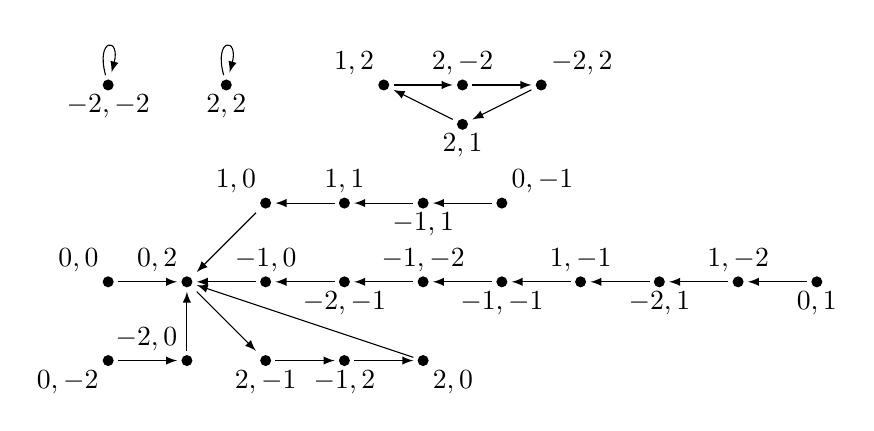
\begin{tikzpicture}[>=latex]
{\centering
\node (-2-2) at (-0.5, 2)    {};
\node (-2-1) at (2.5, -0.5)   {};
\node (-20) at (0.5, -1.5) {};
\node (-1-2) at (3.5, -0.5)   {};
\node (-1-1) at (4.5, -0.5) {};
\node (-10) at (1.5, -0.5)   {};
\node (0-2) at (-0.5, -1.5)   {};
\node (0-1) at (4.5, 0.5) {};
\node (00) at (-0.5, -0.5)    {};
\node (1-2) at (7.5, -0.5) {};
\node (1-1) at (5.5, -0.5)  {};
\node (10) at (1.5, 0.5) {};
\node (2-2) at (4, 2)   {};
\node (2-1) at (1.5, -1.5) {};
\node (20) at (3.5, -1.5) {};

\node (-22) at (5, 2)    {};
\node (-21) at (6.5, -0.5)  {};
\node (-12) at (2.5, -1.5)   {};
\node (-11) at (3.5, 0.5) {};
\node (02) at (0.5, -0.5)   {};
\node (01) at (8.5, -0.5) {};
\node (12) at (3, 2) {};
\node (11) at (2.5, 0.5)   {};
\node (22) at (1, 2)   {};
\node (21) at (4, 1.5) {};

\fill (-2-2)[right] circle (0.07) node[below]       {$-2,-2$};
\fill (-2-1)[right] circle (0.07) node[below]       {$-2,-1$};
\fill (-20)[left] circle (0.07) node[above left]       {$-2,0$};
\fill (-21)[left] circle (0.07) node[below]       {$-2,1$};
\fill (-22)[left] circle (0.07) node[above right]       {$-2,2$};
\fill (-1-2)[left] circle (0.07) node[above]       {$-1,-2$};
\fill (-1-1)[left] circle (0.07) node[below]  {$-1,-1$};
\fill (-10)[left] circle (0.07) node[above]       {$-1,0$};
\fill (-11)[left] circle (0.07) node[below]  {$-1,1$};
\fill (-12)[left] circle (0.07) node[below]  {$-1,2$};
\fill (0-2)[left] circle (0.07) node[below left]  {$0,-2$};
\fill (0-1)[left] circle (0.07) node[above right]       {$0,-1$};
\fill (00)[left] circle (0.07) node[above left]       {$0,0$};
\fill (01)[left] circle (0.07) node[below]  {$0,1$};
\fill (02)[left] circle (0.07) node[above left] {$0,2$};
\fill (2-2)[right] circle (0.07) node[above]       {$2,-2$};
\fill (2-1)[right] circle (0.07) node[below ]       {$2,-1$};
\fill (20)[left] circle (0.07) node[below right]       {$2,0$};
\fill (21)[left] circle (0.07) node[below]       {$2,1$};
\fill (22)[left] circle (0.07) node[below]       {$2,2$};
\fill (1-2)[left] circle (0.07) node[above]       {$1,-2$};
\fill (1-1)[left] circle (0.07) node[above]  {$1,-1$};
\fill (10)[left] circle (0.07) node[above left]       {$1,0$};
\fill (11)[left] circle (0.07) node[above]  {$1,1$};
\fill (12)[left] circle (0.07) node[above left]  {$1,2$};

%>>> def f(x1, x2):
%...     y = (x2 + 2 * x1 * x2 + 2) % 5
%...     return y if y < 3 else y - 5

%>>> d = {(x, y): (y, f(x, y)) for x in range(-2, 3) for y in range(-2, 3)}
%>>>for k in d:
%...     if k == d[k]:
%...             print('\path[->]', k, 'edge [loop above] node {} ();')
%...     else:
%...             print('\path[->]', k, 'edge node {}', d[k], ';')

\path[->] (-2-2) edge [loop above] node {} ();
\path[->] (-2-1) edge node {} (-10) ;
\path[->] (-20) edge node {} (02) ;
\path[->] (-21) edge node {} (1-1) ;
\path[->] (-22) edge node {} (21) ;
\path[->] (-1-2) edge node {} (-2-1) ;
\path[->] (-1-1) edge node {} (-1-2) ;
\path[->] (-10) edge node {} (02) ;
\path[->] (-11) edge node {} (11) ;
\path[->] (-12) edge node {} (20) ;
\path[->] (0-2) edge node {} (-20) ;
\path[->] (0-1) edge node {} (-11) ;
\path[->] (00) edge node {} (02) ;
\path[->] (01) edge node {} (1-2) ;
\path[->] (02) edge node {} (2-1) ;
\path[->] (1-2) edge node {} (-21) ;
\path[->] (1-1) edge node {} (-1-1) ;
\path[->] (10) edge node {} (02) ;
\path[->] (11) edge node {} (10) ;
\path[->] (12) edge node {} (2-2) ;
\path[->] (2-2) edge node {} (-22) ;
\path[->] (2-1) edge node {} (-12) ;
\path[->] (20) edge node {} (02) ;
\path[->] (21) edge node {} (12) ;
\path[->] (22) edge [loop above] node {} ();

}
\end{tikzpicture}

В случае $\gamma = (2, 2)$ последовательность оказывается полностью состоящей из двоек, поэтому период такой последовательности будет равен единице.

\task{Над полем $GF(2)$ построить ЛРП периода $T$ и ранга $n$ и указать начальное заполнение.

$T = 84, n = 8.$
}

Разложим $T$ на множители: $T = 84 = 4 \cdot 3 \cdot 7$. 

ЛРП$_1$ c периодом 4 соответствует минимальный многочлен
$$f_1 (x) = x^3 + x^2 + x + 1,\ x_i = x_{i-1} + x_{i-2} + x_{i-3}.$$

ЛРП$_2$ с периодом 3 соответствует минимальный многочлен
$$f_2 (x) = x^2 + x + 1,\ x_i = x_{i-1} + x_{i-2}.$$

ЛРП$_3$ с периодом 7 соответствует минимальный многочлен
$$f_3 (x) = x^3 + x + 1,\ x_i = x_{i-2} + x_{i-3}$$

Искомый характеристический многочлен
$$f(x) = (x^3 + x^2 + x + 1)(x^2 + x + 1)(x^3 + x + 1) = x^8 + x^4 + x^3 + x^2 + x + 1.$$

Характеристическое уравнение будет иметь вид:
$$x_i = x_{i-4} + x_{i-5} + x_{i-6} + x_{i-7} + x_{i-8}.$$

Выберем начальные заполнения для ЛРП$_{1-3}$, отличные от нуля, и получим первые начальные отрезки ЛРП длины $n=8$:
$$\widetilde \alpha _1 = 001 \Rightarrow \widetilde \beta _1 = 00110011$$
$$\widetilde \alpha _2 = 01 \Rightarrow \widetilde \beta _2  = 01101101$$
$$\widetilde \alpha _3 = 001 \Rightarrow \widetilde \beta _3 = 00101110$$

Искомое начальное заполнение:
$$\widetilde \beta = \widetilde \beta _1 \oplus \widetilde \beta _2 \oplus \widetilde \beta _3 = 01110000.$$

Ответ: $f(x) = x^8 + x^4 + x^3 + x^2 + x + 1$, $\widetilde \beta = 01110000$. 
